\documentclass{article}
\usepackage{amsmath,amssymb}
\usepackage{tikz}
\usepackage{pgfplots}
\usepackage{hyperref}
\usepackage{graphicx}
\usepackage{xcolor}

\title{Sample \LaTeX{} Article with Math and TikZ}
\author{GitHub Actions Demo}
\date{\today}

\begin{document}

\maketitle

\begin{abstract}
  This is a sample \LaTeX{} article that demonstrates the automatic conversion to HTML using GitHub Actions. It includes mathematical equations and TikZ diagrams to showcase the capabilities of the conversion process.
\end{abstract}

\section{Introduction}

This document serves as a demonstration of the automatic \LaTeX{} to HTML conversion process using GitHub Actions. The workflow uses \texttt{make4ht} with MathJax and SVG output to create a standalone HTML website from this \LaTeX{} source.

\section{Mathematical Equations}

Here are some examples of mathematical equations that will be rendered using MathJax:

\subsection{Inline Math}

The quadratic formula is $x = \frac{-b \pm \sqrt{b^2 - 4ac}}{2a}$ for a quadratic equation $ax^2 + bx + c = 0$.

\subsection{Display Math}

The famous Euler's identity:
\begin{equation}
  e^{i\pi} + 1 = 0
\end{equation}

A more complex equation:
\begin{align}
  \int_{-\infty}^{\infty} e^{-x^2} \, dx &= \sqrt{\pi} \\
  \sum_{n=0}^{\infty} \frac{1}{n!} &= e \\
  \prod_{i=1}^{n} i &= n!
\end{align}

A matrix example:
\begin{equation}
  A = \begin{pmatrix}
    a_{11} & a_{12} & \cdots & a_{1n} \\
    a_{21} & a_{22} & \cdots & a_{2n} \\
    \vdots & \vdots & \ddots & \vdots \\
    a_{m1} & a_{m2} & \cdots & a_{mn}
  \end{pmatrix}
\end{equation}

\section{TikZ Diagrams}

Here are some examples of TikZ diagrams that will be converted to SVG:

\subsection{Simple Shapes}

\begin{figure}[h]
  \centering
  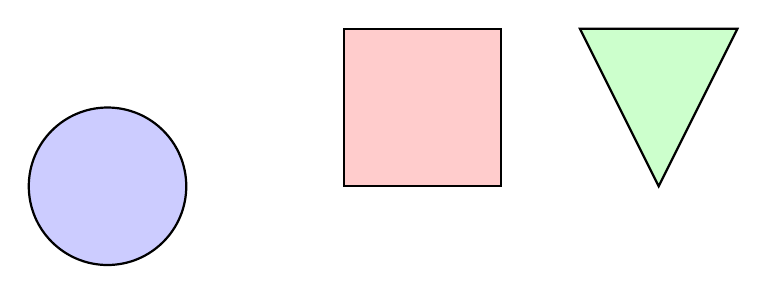
\begin{tikzpicture}
    \draw[thick, fill=blue!20] (0,0) circle (1cm);
    \draw[thick, fill=red!20] (3,0) rectangle (5,2);
    \draw[thick, fill=green!20] (7,0) -- (8,2) -- (6,2) -- cycle;
  \end{tikzpicture}
  \caption{Basic shapes in TikZ: circle, rectangle, and triangle}
\end{figure}

\subsection{Function Plot}

\begin{figure}[h]
  \centering
  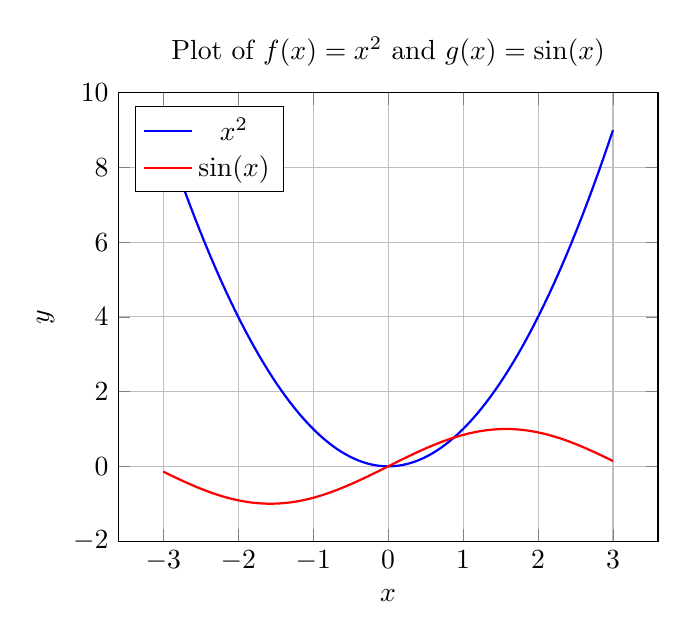
\begin{tikzpicture}
    \begin{axis}[
      xlabel={$x$},
      ylabel={$y$},
      title={Plot of $f(x) = x^2$ and $g(x) = \sin(x)$},
      legend pos=north west,
      grid=both,
      domain=-3:3,
      samples=100
    ]
      \addplot[blue, thick] {x^2};
      \addplot[red, thick] {sin(deg(x))};
      \legend{$x^2$, $\sin(x)$}
    \end{axis}
  \end{tikzpicture}
  \caption{Function plots using PGFPlots}
\end{figure}

\subsection{Flowchart}

\begin{figure}[h]
  \centering
  \begin{tikzpicture}[node distance=2cm, auto]
    % Define styles
    \tikzstyle{decision} = [diamond, draw, fill=blue!20, text width=4.5em, text badly centered, inner sep=0pt]
    \tikzstyle{block} = [rectangle, draw, fill=blue!20, text width=5em, text centered, rounded corners, minimum height=4em]
    \tikzstyle{line} = [draw, -latex']
    
    % Place nodes
    \node [block] (init) {Initialize};
    \node [block, below of=init] (process) {Process};
    \node [decision, below of=process] (decide) {Decision?};
    \node [block, below left of=decide, xshift=-1.5cm] (yes) {Yes};
    \node [block, below right of=decide, xshift=1.5cm] (no) {No};
    \node [block, below of=yes, xshift=1.5cm] (end) {End};
    
    % Connect nodes
    \path [line] (init) -- (process);
    \path [line] (process) -- (decide);
    \path [line] (decide) -- node [near start] {yes} (yes);
    \path [line] (decide) -- node [near start] {no} (no);
    \path [line] (yes) |- (end);
    \path [line] (no) |- (end);
  \end{tikzpicture}
  \caption{A simple flowchart using TikZ}
\end{figure}

\section{Conclusion}

This sample document demonstrates how \LaTeX{} documents with mathematical equations and TikZ diagrams can be automatically converted to HTML using GitHub Actions. The resulting HTML will use MathJax for rendering equations and SVG for the TikZ diagrams, ensuring high-quality display across different devices and browsers.

The GitHub Actions workflow handles the conversion process, organizes the output files, and deploys everything to GitHub Pages, making it easy to share your \LaTeX{} documents on the web.

\end{document}